\chapter{Introduction to Reinforcement Learning}
When I say “autonomous network,” I don’t just mean “it runs without me pushing buttons.” I mean a communication system that behaves like an independent organism: it senses what’s happening, it reasons about what to do, it acts, and it improves over time. 

\begin{redbar}
An autonomous network requires \textbf{intelligence}: the ability to learn from the local environment and to change behavior when conditions change. That could be a squad of drones routing messages among themselves, or a home full of tiny devices that wake up and speak only when they have something new to say.
\end{redbar}

We’re going to focus on autonomy at the networking level — that is, how nodes communicate and route information. The central question is: how do we make a distributed system of devices behave intelligently without constant human configuration?

Autonomy in networking shows up in many wireless domains. Think about sensor networks and IoT, backscatter/RFID systems, and drone networks. These examples share a few traits: many small devices, limited energy budgets, event-driven data, and a wireless medium that is noisy and shared. Each environment raises specific constraints and opportunities for autonomy.

A particularly revealing example is the battery-free smart home. That setting is useful because it stretches a designer’s constraints: devices cannot carry batteries, so they must harvest energy; sensors are heterogeneous (cameras, temperature probes, presence detectors, remotes, switches); and data arrival is highly irregular — sometimes bursty, sometimes sparse, sometimes continuous.
The peculiarities of battery-free devices change how we design the network:
\begin{itemize}
    \item First, devices produce data with very different timing characteristics. A joystick or remote produces bursts only when a user interacts. A temperature sensor usually updates slowly, but during a fire it will produce urgent, rapid updates. Presence sensors are silent until someone walks by. A camera, by contrast, produces continuous high data volume.
    \item Second, these devices cannot transmit whenever they like. In backscatter systems, a reader must query a tag to provide the energy and the “opportunity” to transmit. That means the reader controls when devices can speak.
    \item Third, we’d like two things at once: ask a tag only when it actually has new data (avoid wasted queries), and make sure we don’t miss data that was produced between queries (avoid data loss).
\end{itemize}
A natural approach is TDMA: give each tag a fixed timeslot and cycle through them. Another is random access (e.g., ALOHA-style), where tags reply opportunistically. Both have problems in battery-free backscatter environments.
With random access, simultaneous replies collide because many tags share the same short window to backscatter. Collisions mean wasted energy and lost packets — bad when the reader’s energy budget matters.
With TDMA fixed assignment, a tag may be polled repeatedly even when it has nothing new to report. That wastes the reader’s time and the tiny energy budget available to tags (they must harvest enough energy during that timeslot to sense and reply). Worse, if a device produces new data twice between its assigned slots, the older sample might get overwritten or lost before it’s ever reported.

Our aim is a MAC protocol that adapts autonomously with two practical goals:
\begin{enumerate}
    \item Query devices only when they are likely to have new data, minimizing wasted queries.
    \item Avoid losing data due to infrequent polling, so fresh samples are delivered within acceptable delay.
\end{enumerate}
So how can a single reader learn which devices to poll and when? The answer in this context is to learn from experience: observe which polling choices lead to useful data and which don’t, and adjust the policy accordingly. That learning-by-interaction approach is exactly what reinforcement learning (RL) provides.

\textit{Reinforcement learning} is about learning what to do through trial and error. An RL agent doesn’t get told the correct action; instead it takes actions and receives feedback in the form of rewards or penalties. Over time the agent learns which actions tend to lead to high cumulative reward.

Crucially, RL handles sequential decision making: your current action affects not only the immediate reward but the future state and future rewards.

Three core pieces make up an RL setup: \textit{sensation} (what the agent observes about the world), \textit{action} (what the agent can do), and \textit{goal} (the reward it is trying to maximize).

There are a few things that separate RL from other machine learning approaches, and those differences make RL attractive here.
\begin{enumerate}
    \item First, there is no supervisor giving the “right” action. You don’t have labeled data saying “this tag should have been polled now.” You only have a signal: the poll either returned fresh data or it didn’t.
    \item Second, feedback can be delayed. Choosing to poll tag A now might prevent polling tag B until later, causing B’s next sample to be lost — a bad outcome that’s only apparent later. RL handles these delayed consequences naturally because it optimizes for cumulative reward, not immediate gains.
    \item Third, actions change the data stream the agent receives. If the reader polls a device frequently, it will see a steady stream of data from that device; if it ignores it, the device’s samples may pile up or be dropped, changing future observations.
    \item Finally, RL naturally supports online learning. We don’t want to train the reader offline and freeze it: device populations and human habits change.
\end{enumerate}
As an example, think of an infant waving its arms. There is no supervisor telling the baby what each motion will cause, but the baby quickly learns — some motions cause attention, others cause objects to fall. Through many small trials and the consequences that follow, the infant builds a sense of cause and effect.
The reader similarly must “experiment.” It will poll devices it suspects have new data, learn which polling patterns work, and gradually improve. Early on there will be mistakes: wasted polls and maybe missed samples. A robust RL formulation minimizes the long-term cost of those mistakes and keeps exploring enough to adapt to changes.

\section{Applications of Reinforcement Learning}
Reinforcement learning powers real systems you’ve heard of and many you haven’t. 
\begin{itemize}
    \item Think about self-driving cars: beyond end-to-end perception, RL can be used to optimize trajectories, plan motions, choose dynamic lanes on a crowded highway, tune low-level controllers, or learn policies for specific highway scenarios where rules and interactions are complicated. 
    \item In factories and industrial automation RL drives robots that do repetitive, heavy, or hazardous work more efficiently than people and sometimes in ways people can’t (or shouldn’t) do themselves.
    \item In healthcare, clinical decisions and treatments often have delayed outcomes: the effect of a medication may be visible only days or months later. RL can learn policies from past patient trajectories — without requiring a perfect mathematical model of human biology — and, when carefully validated, propose treatment schedules that maximize long-term patient outcomes rather than immediate, short-term metrics.
    \item Facebook (now Meta) developed Horizon, an open-source RL platform, and has applied RL to personalize suggestions, choose which notifications matter, and even improve video streaming quality by learning policies at scale. 
    \item News recommendation and ad bidding are natural RL playgrounds because user preferences change quickly; an RL system can adapt recommendations by observing how users return or engage after each suggestion. 
\end{itemize}
And beyond these examples, RL plays roles in finance and trading, natural language processing (e.g., optimizing dialogue policies), gaming and simulation, robotics, real-time bidding, and, importantly for our course, computer networking: routers, schedulers, and MAC protocols can all learn better policies from interaction.

\section{Rewards}
At the heart of RL is the reward. The \textit{reward} at a single time step, call it $R_t$, is just a scalar number the environment hands back to the agent after it takes an action. That number is the agent’s only direct signal about how well it’s doing at that moment. The agent’s objective is to maximize cumulative reward over time, not just instant reward.

There’s also the reward hypothesis: the informal claim that any goal can be represented as maximizing expected cumulative reward. That hypothesis is useful as a unifying idea — if you can design a reward function that captures what you want, RL will try to optimize it — but it’s also a caution.
Examples help make reward design concrete. 
\begin{itemize}
    \item Suppose you want a humanoid robot to walk forward. The reward design can be simple: give positive reward for forward displacement and a steep negative penalty if the robot falls. The positive reward encourages movement in the desired direction; the negative penalty prevents the agent from exploiting the positive reward by adopting unstable gaits that produce forward motion only briefly and then crash.
    \item Now imagine a helicopter learning stunt maneuvers. The helicopter should be rewarded for tracking a desired trajectory (following the planned path) and heavily penalized for crashing.
    \item Translate the same idea to communication in battery-free environments. A sensible reward might give a positive value when a query returns new sensor data and a negative value when a query finds nothing or when a sample is lost due to long polling intervals.
\end{itemize}
RL is a framework for sequential decision making. The action you pick now can influence what states and rewards you see later, sometimes dramatically. That’s why RL optimizes expected cumulative reward rather than immediate payoff.
Sometimes you should sacrifice a small immediate reward to unlock a large reward later.

\section{The exploration–exploitation dilemma}
A central conundrum in RL is the \textit{exploration–exploitation} trade-off. To collect reward you want to pick actions that you already know to be good — \textit{exploit}. But to discover possibly better actions you need to try things you haven’t tried yet — \textit{explore}. If you exploit too much you may get stuck in a locally optimal but globally subpar strategy. If you explore too much you waste opportunities that you could have turned into reward.

As a simple life example: your favorite restaurant sits around the corner. If you eat there every day you get consistent meals you like — low risk, reliable reward. But you’ll never learn whether an even better place exists. If, instead, you try a new restaurant every lunch you might uncover better food, but you’ll also suffer more bad meals along the way. The best long-term strategy typically mixes both behaviors: exploit often but keep trying new places occasionally to discover surprises.

In a stochastic environment, the same action can give different outcomes each time; to estimate an action’s true value you must try it many times. That requirement is costly when trials are expensive (physical robots with wear and tear), slow (medical trials), or risky (a policy that could cause a crash or safety violation).

The exploration–exploitation problem has been studied for decades and remains a central challenge because there is no single perfect strategy that works in every domain.

\section{General RL framework}
The general RL framework picture a simple loop: there’s an agent and there’s an environment (see Figure \ref{fig:agent}). At each step the agent chooses an action and the environment responds by handing back two things — an observation and a scalar reward. We usually write the action at time $t$ as $A_t$, the observation as $O_t$, and the reward as $R_t$. Time progresses in discrete environment steps, and every step repeats that same handshake: agent acts, environment replies.

\begin{figure}[ht]
    \centering
    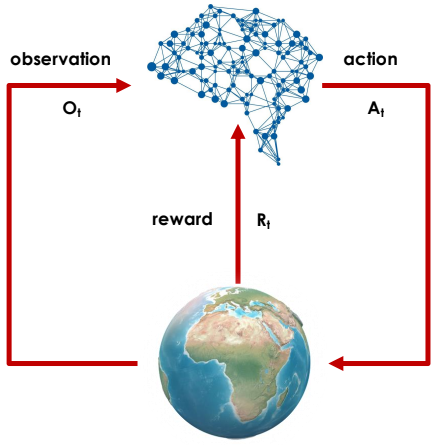
\includegraphics[width=0.5\linewidth]{images/agent.png}
    \caption{Agent and environment.}
    \label{fig:agent}
\end{figure}

That handshake is the foundation of reinforcement learning. The agent never sees the “internal wiring” of the environment; it only sees the observations and rewards that the environment emits and then must act on those signals.

Everything the agent has ever observed, done, and received up to time $t$ can be collected into a single object called the \textit{history}. Formally the history at time $t$ is 
\begin{equation*}
    H_t=A_1,O_1,R_1,\ldots,A_t,O_t,R_t,    
\end{equation*}
which is simply the full stream of action taken, observation perceived, and reward obtained.
That sequence is important because what happens next generally depends on the entire history. In practice, however, the agent doesn’t need to reason over the whole raw history every moment. Instead we define a \textit{state} as any function of the history that contains the information needed to predict what comes next. More compactly,
\begin{equation*}
    S_t=f(H_t),    
\end{equation*}
where $f$ is some mapping that extracts the relevant information from the history. That mapping can be as simple as the last observation, a short window of recent observations, or a complicated belief distribution over hidden environment variables.

Two complementary notions of state matter. The environment has its own private state, call it $S_t^e$, which the environment uses internally to determine the next observation and the reward. The agent has an internal representation — its agent state, call it $S_t^a$ — which is the information the agent actually uses when picking its next action. The environment’s state $S_t^e$ is generally not directly visible to the agent; the agent must infer or represent what it thinks the environment state might be from its history. The agent internal representation $S_t^a$ is the information used by reinforcement learning algorithms. It can be any function of history:
\begin{equation*}
    S_t^a = f(H_t)
\end{equation*}
If the agent state equals the environment state, we say the problem is \textit{fully observable}: whatever the environment uses to decide the next outcome is available to the agent. In that ideal world you can, in principle, make optimal decisions because you can see exactly what matters.

Reality is usually messier. In many practical tasks the agent only sees part of the environment. A robot with a camera doesn’t receive the robot’s absolute coordinates; a trading agent only sees current market prices and not hidden trader intentions; sensors in a house only report local measurements but not the whole home state. When the agent only has indirect information, the problem is \textit{partially observable}. In these cases the agent must summarize the history into a representation (beliefs, recency statistics, or other features) that helps it to predict future observations and rewards.

An RL agent typically contains three conceptual components that work together.
\begin{enumerate}
    \item \textit{Policy.} The policy is the agent’s behavior function: given the agent’s internal state, the policy decides what action to take. It is the active part of the agent — it produces behavior.

    When we say “policy,” we mean a mapping from the agent’s state to an action. If the mapping is deterministic, the policy returns a single action for each state. If it’s stochastic, the policy returns probabilities for each action — the agent then samples an action according to those probabilities.

    The reward signal is the agent’s only direct evaluation of behavior: when a chosen action is followed by low reward, the policy should update to favor different actions in similar states. The design of how the policy updates depends on the algorithm (policy gradients, Q-learning, actor-critic, etc.), but the conceptual link is the same: reward guides change.
    
    \item \textit{Value function.} Rewards tell you what’s good immediately, but value predicts what’s good in the long run. A value function answers the question “starting from this state, how much cumulative reward can I expect to get if I follow policy X?” That predicted future reward is what lets the agent prefer actions that may pay off later rather than only chasing immediate gains.

    A value function is a prediction. For a policy $\pi$, the state-value function $v_\pi(s)$ is the expected return starting from state  $s$ and following $\pi$ thereafter. If we use the discounted return
    \begin{equation*}
        G_t=R_{t+1}+\gamma R_{t+2}+\gamma^2 R_{t+3}+\ldots,
    \end{equation*}
    then the value is
    \begin{equation*}
        v_\pi(s)=E_\pi[G_t|S_t=s].
    \end{equation*}
    Intuitively, $v_\pi(s)$ tells you how “promising” that state is in terms of future cumulative reward. Even a state with low immediate reward can have high value if it reliably leads to better states later. Value functions are central to many RL algorithms because they reduce long-term optimization to estimating expected sums of rewards.
    
    \item \textit{Model.} A model predicts consequences: given a state and an action, what next observation or next environment state is likely to follow, and what reward can we expect? Models let agents plan by simulating hypothetical futures.

    A model predicts the environment’s reaction to actions. It can give the resultant next state, the expected immediate reward, or both. Model-based agents can use such predictions to plan: they simulate sequences of actions ahead of time to choose those that look best, which can accelerate learning when models are accurate.

    Model-free methods skip building an explicit model and instead directly learn policy or value estimates from transitions observed in the real environment.
\end{enumerate}
